\chapter{Questions difficulty}
During the first public release of Reminisce.me, family and friends were asked to play the game and provide feedback. With the help of the 58 games played, we were able to get information about some important aspects of the game: which questions are selected by the users, are they answering randomly or by thinking, how much time they take to answer the questions. This feedback was really useful to understand how difficult the game was and what kind of improvement has to be made. One of the first issue was that the questions were generated completely randomly and there was no concern about how difficult they were, we mostly used parameters that we thought would make sense and not too difficult. We had two main reasons for wanting to be able to change the difficulty at will.\\
The first and most obvious reason is that it makes the game more enjoyable, getting hard questions and failing over and over is  not amusing and the same goes if you only get easy question which offer no challenge at all. The second reason is that by being able to toy with the difficulty, we can test hypotheses and improve our understanding of memory: if we think that some parameter is a central element of what makes an element memorable we can then consider it when modifying questions' difficulty and see whether or not this affects the results when games are played.\\
It was therefore important to add some modularity to the question generation process and decide what parameters could be played with to influence the difficulty. Note that older events are obviously harder than recent events so we did not take into account the creation date of a post when discussing the difficulty of a question. We approached the problem from two angles, the selection of items and the generation of the question itself.\\
Some items will be harder to remember than others no matter the way the question is then generated. For instance, finding out precisely when something was posted is hard if it is in the middle of a lot of other posts because it was posted during a period of heavy usage of Facebook. On the other hand, isolated posts are really memorable because they are often about something so noteworthy that it made the user go on Facebook and talk about it when they were in the middle of a low usage period.\\
The way items are used when generating questions is also something that increases and decreases difficulty. The choice of other alternatives in a multiple choice questions has a lot of influence on the difficulty and the size of the proposed time periods on a time question has also an influence.

\section{Clustering}
\subsection{Why do we need clustering}
Clustering is a standard data analysis technique. ``[It] is the task of grouping a set of objects in such a way that objects in the same group (called a cluster) are more similar (in some sense or another) to each other than to those in other groups (clusters).''\cite{clustering} It is often used in data mining to perform pattern recognition as it allows to find similar items in a data set. The reason we are using it is that we want to find sets of similar posts or similar pages which are then hard to compare to each other. This is of great help when generating ordering questions as three elements belonging to a same cluster are then harder to cluster than those in different clusters.
\subsection{Algorithm choice}
There are a lot of different algorithms which can achieve clustering. They all have different behaviors and required input. Some of the most common algorithms are k-means and DBSCAN.\\
K-means ``aims to partition n observations into k clusters in which each observation belongs to the cluster with the nearest mean''\cite{kmeans}. The algorithm works quite well when the number of clusters is known in advance and provides a centroid for each cluster which is the mean value for each cluster.\\
``Density-based spatial clustering of applications with noise (DBSCAN) [...] groups together points that are closely packed together (points with many nearby neighbors), marking as outliers points that lie alone in low-density regions (whose nearest neighbors are too far away).''\cite{dbscan} This algorithm does not provide centroids but has the nice property to discover the right number of cluster by itself based on the density of the data set.\\
Figure \ref{fig:clustComp} shows a visual representation of the results of different variations of k-means and DBSCAN when applied to the same datasets. One can see that k-means works well when the number of expected clusters is the same as the number of clusters that the data set has. However, when the data set has a different number of cluster or their shape is such that one cannot enclose them in separate circles, the results are less than convincing. On the other hand DBSCAN behaves well in all those cases.\\
In our application, we do not know the number of clusters in advance, it is something we would like the algorithm to help us discover, therefore the choice was to use DBSCAN.

\begin{figure}
\centering
{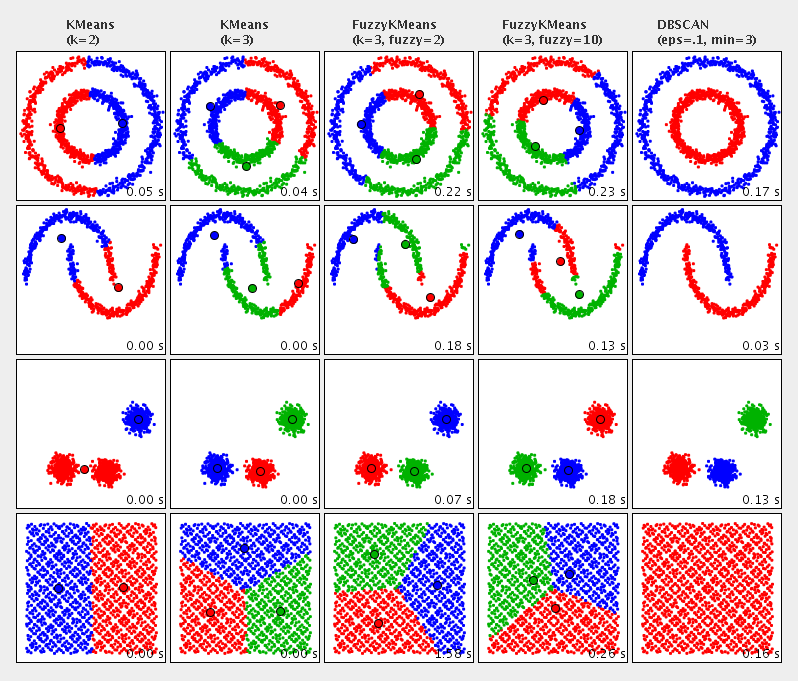
\includegraphics[width=6in]{images/cluster_comparison.png}}
\caption{Comparison of multiple clustering techniques \cite{apachecluster}}
\label{fig:clustComp}
\end{figure}

\section{How does DBSCAN work}
\subsection{General notions}
Besides the data set, DBSCAN works with two parameters as inputs, $\epsilon$ and $minPts$. $\epsilon$ can be seen as a density measure, it is the distance between two points which we would consider acceptable for them to be in the same cluster. $minPts$ is the minimum number of points in a cluster.\\
Let's introduce a few notions\cite{dbscan}:
\begin{itemize}
	\item A \emph{core point} is point which is surrounded by at least $minPts$ points within a distance of $\epsilon$. Those points are said to be \emph{directly reachable} from this \emph{core point}. By definition, no points are \emph{directly reachable} from a non-core point.
	\item A point $q$ is said to be \emph{reachable} from a core point $p$ if there is a sequence of points, all \emph{directly reachable} from the previous one, which starts at $p$ and ends at $q$. All those points must be \emph{core points} except $q$.
	\item All non-core, non-reachable points are \emph{outliers}
	\item Two points $p$ and $q$ are \emph{density connected} if there is a point $o$ from which they are both \emph{reachable}
\end{itemize}

And then the points in a cluster satisfy the following properties\cite{dbscan}:
\begin{itemize}
	\item All points within the cluster are mutually density-connected.
	\item If a point is \emph{reachable} from any point of the cluster, it is part of the cluster as well.
\end{itemize}

Figure \ref{fig:reachExample} illustrates those definitions.

\begin{figure}
\centering
{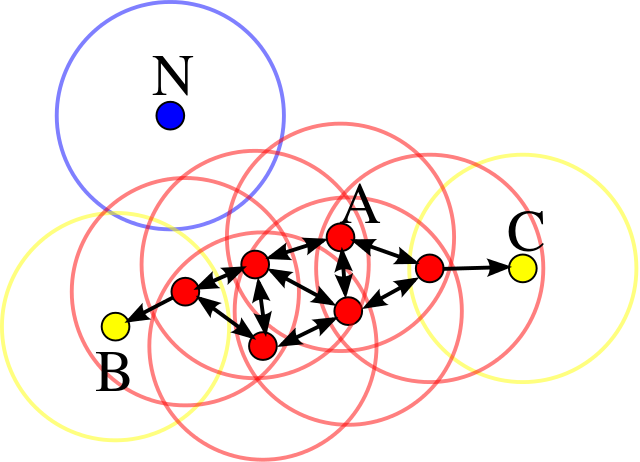
\includegraphics[width=3.5in]{images/reach_example.png}}
\caption{This figure taken from \cite{dbscan} shows an example where $minPts=4$. $\epsilon$ is represented by the circles. The points in red are \emph{core points}, the ones in yellow are \emph{reachable} and the one in blue is an outlier. The cluster would be comprised of points in red and yellow.}
\label{fig:reachExample}
\end{figure}

\subsection{The algorithm itself}

Let's first define the $\epsilon$-\emph{neighborhood} of a point as the set of points which are at a distance less than $\epsilon$ from this point. The algorithm works ass follows\cite{dbscan}:
\begin{enumerate}
	\item \label{initdbscan} Pick a point $P$ that was not visited yet from the data set and mark $P$ as visited. If no such point exists, the algorithm is completed.
	\item Let $N$ be the $\epsilon$-\emph{neighborhood} of this point. If $N$ contains at least $minPts$ points, $P$ is a \emph{core point}. In that case create a new cluster $C$ containing only $P$, otherwise go back to \ref{initdbscan}.
	\item All the points in $N$ should obviously be part of cluster $C$aw as they are neighbors of a \emph{core point} ($P$) and are at a distance less than $\epsilon$ from this point. We must include them in the cluster, but if those points are also \emph{core points} we must also include their neighborhoods and so on (forming sequences of \emph{core points} to find all the \emph{reachable} points). To achieve this, we will remember all the points we have to visit in a set we will call $V$. First, put all the points from $N$ in $V$ then go to \ref{loopdbscan}.
	\item \label{loopdbscan} Pick a point $P'$ in $V$ that was not visited and mark $P'$ as visited. If no such point exists, go to \ref{initdbscan}.
	\item If $P'$ does not belong to any cluster yet, add $P'$ to cluster $C$.
	\item If the $\epsilon$-\emph{neighborhood} of $P'$ contains at least $minPts$ points, add the $\epsilon$-\emph{neighborhood} of $P'$ to $V$. Go to \ref{loopdbscan}.
\end{enumerate}

At the end, all the points which are not in any cluster are \emph{outliers}.

\subsection{Parameters selection}

\section{Multiple Choice Questions}
Use of relationship between the users.
\section{Ordering Questions}
Reactions: standard deviation from the mean.
Pages: clustering: in same cluster -> hard, two clusters -> easy, cluster + non-cluster -> medium
\section{Geolocation Questions}
Cluster: in a large cluster -> easy, outside of cluster -> hard, in medium sized cluster -> medium
\section{Timeline questions}
Same as geolocation.
\section{Difficulty selection}